The purpose of this chapter is to explain concepts and sensors referenced later in the report, and to describe the functionality of the sensors and hardware used in the DAQ package.
An overview of SDM-22's DAQ package has also been included for reference.
\section{Previous Design}
The DAQ package for SDM-22 was a complete overhaul of previous DAQ packages designed and manufactured by the team.
The SDM-22 DAQ package's goal was to create a permanent DAQ presence on the vehicle.
For instance this included permanent mounting spots in the vehicle for DAQ boxes.
Additionally printed circuit boards were designed for the first time to simplify wiring within each box.
A Teensy 4.1 microcontroller replaced the Arduino Mega as the main board, due to its smaller form factor, additional hardware features such as CAN and more Serial and I2C ports, as well as the built in micro SD card socket.
Teensy 4.0 microcontrollers were used for auxiliary data hubs, whose purpose were to collect data from local sensors and transmit them back to the main board.
\vspace{1em}

Although the SDM-22 DAQ package made big improvements to previous iterations, it was not without faults.
The wire connectors used in the package were difficult to use, and the system was not able to retrieve CAN data from the ECU, possibly due to a faulty CAN transceiver board.
Serial communication between the main board and data hubs were also slow at around 8 packets transmitted per second, likely due to needlessly large data packets.
Additionally, the planning and designs of the mounting solutions for the boxes were held back by the electrical design, resulting in a non-optimal mounting place for the main board.

\section{Selected Components}
The components discussed in this section are the sensors and other hardware that have been included in the DAQ package for SDM-23.

\subsection{Primary Microcontroller}
The DAQ package requires sensor processing and communication standards to reliably collect and log data from the vehicle.
The Teensy 4.1 in Figure \ref{fig:t41} is an ARM Cortex-M7 based development board with an NXP iMXRT1062 chip operating at 600 MHz.
Notably it comes with a built-in micro SD socket, 3 CAN controllers, 3 I2C and 8 Serial ports and 18 analog input pins among many other features.
This makes it a great option to use as the main data logger.
\begin{figure}[H]
        \centering
        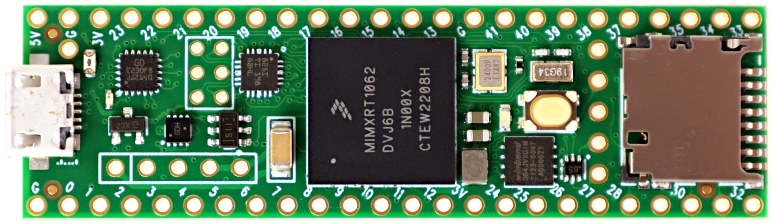
\includegraphics[width=4in]{images/teensy41.jpg}
        \caption{Teensy 4.1 Microcontroller}
        \label{fig:t41}
\end{figure}

\subsection{Auxiliary Microcontroller}
The Teensy 4.0 (Figure \ref{fig:t40}) has the same processing specs as the Teensy 4.1, but in a smaller form factor.
As such, there is less accessible GPIO pins available and no built-in SD socket.
With that said, it still has 7 Serial and 3 I2C ports, 3 CAN controllers, and 14 analog input pins, though some are not as accessible.
\vspace{1em}

%Its smaller form factor makes it a good choice for smaller data hubs that can be placed around the car.
\begin{figure}[H]
\centering
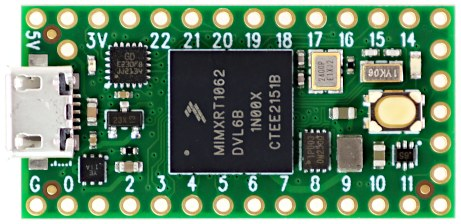
\includegraphics[width=2.2in]{images/teensy40.jpg}
\caption{Teensy 4.0 Microcontroller}
\label{fig:t40}
\end{figure}
\subsection{CAN Transceiver}
To collect data from multiple points on the car into a central location, a robust communication protocol must be implemented.
One such protocol is a Controller Area Network (CAN) bus, which is a standard in the automotive industry designed to allow devices to communicate with each other without a host system.
Devices are connected to each other via a CAN high and CAN low cable, and the network is terminated on both ends by a $120\Omega$ resistor to reduce reflections in the signal.
Each message frame has an ID to determine its priority on the bus.

\begin{figure}[H]
        \centering
        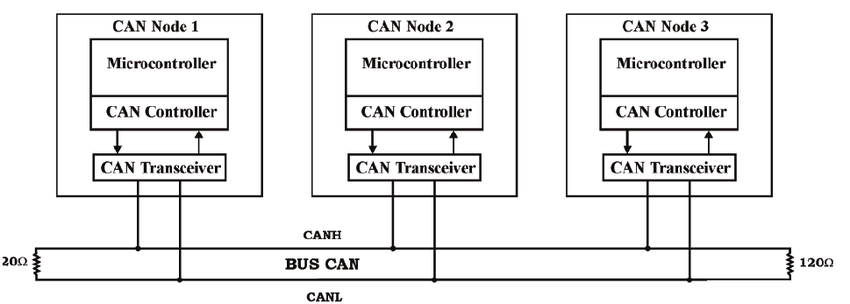
\includegraphics[width=5in]{images/iso11898-can.png}
        \caption{Diagram of a CAN bus}
        \label{fig:can-diagram}
\end{figure}
Both the Teensy 4.0 and 4.1 have a CAN controller in their chip, so to complete the CAN node only a CAN transceiver is needed for each board. This converts the data streams from the CANH and CANL to levels that the CAN controller can use. When transmitting messages the transceiver converts data streams from the controller to the CAN bus levels.
\vspace{1em}

The transceiver chosen is Texas Instruments' SN65HVD230.
It was chosen because it operated on a 3.3V level and would be able to process data from the CAN bus at 1 Mbps, which is the speed at which the Haltech ECU operates at.
This will be used to communicate with the Haltech ECU as well as within the DAQ package.
\begin{figure}[H]
        \centering
        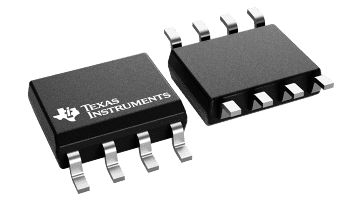
\includegraphics[width=2in]{images/sn65hvd230chip.png}
        \caption{SN65HVD230 CAN Transceiver}
        \label{fig:sn65hvd230}
\end{figure}

\subsection{Linear Potentiometer}
Potentiometers are three-terminal resistors with a sliding or rotating contact that form an adjustable voltage divider.
Linear potentiometers are mounted to SDM-23's suspension in order to measure the damper travel.
Some applications of this data include calculating damper speed and estimating downforce.
\vspace{1em}

The SparkFun X-Large Slide Pot was chosen, primarily because the team already has many in stock and prior success with it.
Although we considered purchasing new linear potentiometers such as the one offered by FSAEparts.com or Haltech, we opted against it as purchasing four of these would be expensive and irresponsible given the other needs of the data acquisition budget.
\begin{figure}[H]
        \centering
        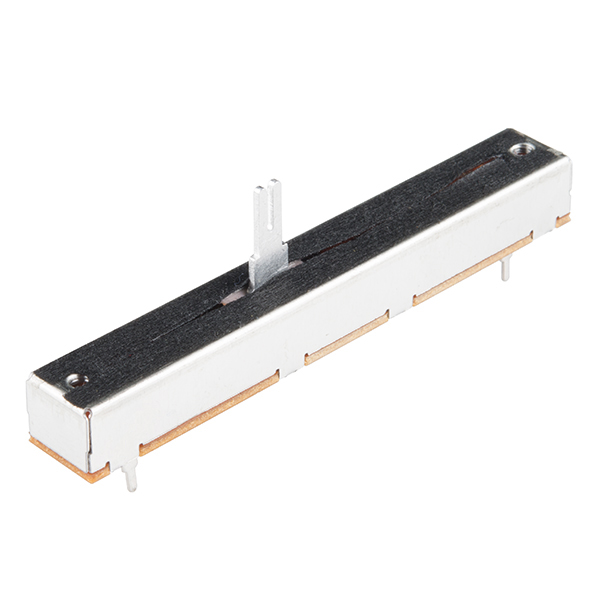
\includegraphics[width=2in]{images/slidepot.jpg}
        \caption{SparkFun X-Large Slide Pot}
        \label{fig:slidepot}
\end{figure}

\subsection{Rotary Potentiometer}
A rotary potentiometer is attached at the pinion gear of the steering rack to measure the steering wheel angle.
A 360-degree rotation potentiometer from CTS was chosen, as we did not want to deal with any interference between the steering wheel rotation and a potentiometer's hard stop.
\begin{figure}[H]
        \centering
        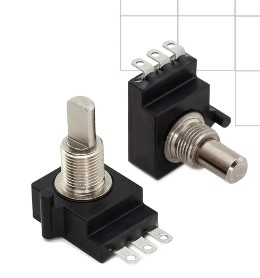
\includegraphics[width=2in]{images/pot.jpg}
        \caption{CTS Rotary Potentiometer}
        \label{fig:pot}
\end{figure}
Other options for measuring rotation include an encoder or a hall effect absolute position sensor.
Encoders are not as viable because of their reduced resolution when compared to a potentiometer, and a hall-effect based position sensor was not chosen as the team has not used them before and mounting it would be much more difficult.
\subsection{6 DoF IMU}
A 6 DoF Inertial Measurement Unit (IMU) is used to measure SDM-23's acceleration and angular velocity on 3 axes.
The module used is ST's ISM330DHCX, which is a high-performance 3D digital accelerometer and gyroscope in a single package.

The SparkFun Breakout board is used and pictured in Figure \ref{fig:ism330dhcx}.
\begin{figure}[H]
        \centering
        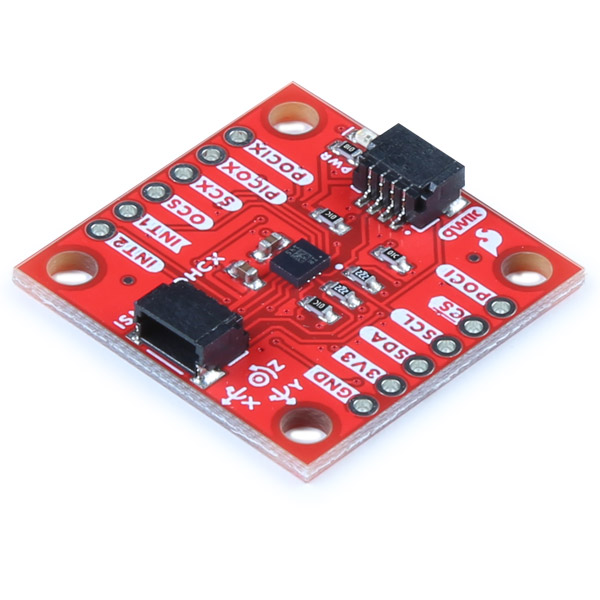
\includegraphics[width=2in]{images/6DoFIMU_03a.jpg}
        \caption{SparkFun ISM330DHCX Breakout Board}
        \label{fig:ism330dhcx}
\end{figure}
Since the Suspension subteam is interested in angular position, the angular velocity data must be integrated to produce position data.

\subsection{Infrared Temperature Sensor}
A MLX90614, an infrared thermometer, is used to measure the rotors' temperatures.
It is an I2C device that operates on 3.3V and can measure an object's temperature up to $380^\circ$C.
Additionally, we are also able to set the emissivity of the object whose temperature we are measuring.
\begin{figure}[H]
        \centering
        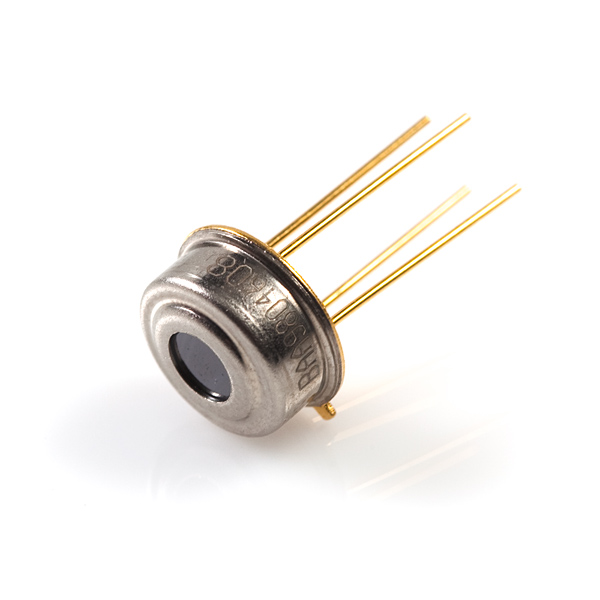
\includegraphics[width=2in]{images/mlx90614.jpg}
        \caption{MLX90614 IR Thermometer}
        \label{fig:mlx90614}
\end{figure}
One downside to infrared sensors is that they are susceptible to sunlight.
Despite this, infrared temperature sensors are still reliable for measuring brake rotor temperatures.


\subsection{Strain Gauge}
Strain gauges are attached to the push and pull rods of SDM-23's suspension.
They are able to measure strain. Using the relationship between strain and stress we can measure the loads that the push and pull rods are subject to.
\begin{figure}[H]
        \centering
        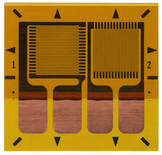
\includegraphics[width=2in]{images/Strain Gauge/125UTA.png}
        \caption{Tee Rosettes Strain Gauge: 125UTA}
        \label{fig:Tee Rosette Strain Gauge: 125UTA}
\end{figure}

Electrically, strain gauges are resistors whose resistance changes based on how they deform.
This resistance change can be measured by a Wheatstone bridge.
\vspace{1em}

Tee rosettes from Micro Measurements were chosen, because its pattern allows us to compensate for temperature without bonding an additional strain gauge, helping us save cost. Shown below are the governing equations. Where G is Shear modulus, E is Young's modulus, $\nu$ is Poisson's Ratio, $\varepsilon$ is strain, $\sigma$ is stress, $\gamma$ is shear strain, and $\tau$ is shear stress. 
\vspace{1em}

\begin{center} 
$[\sigma]_{xyz} = \begin{bmatrix}
\sigma_{xx} & \sigma_{xy}  & \sigma_{xz} \\
\sigma_{yx} & \sigma_{yy}  & \sigma_{yz} \\
\sigma_{xz} & \sigma_{yz}  & \sigma_{zz} 
\end{bmatrix}$ = 
$\begin{bmatrix} \sigma_{xx} & \tau_{xy}  & \tau_{xz} \\
\tau_{yx} & \sigma_{yy}  & \tau_{yz} \\
\tau_{xz} & \tau_{yz}  & \sigma_{zz} 
\end{bmatrix}$
\hspace{0.5cm} \& \hspace{0.5cm}
$[\varepsilon]_{xyz} = \begin{bmatrix}
\varepsilon_{xx} & \varepsilon_{xy}  & \varepsilon_{xz} \\
\varepsilon_{yx} & \varepsilon_{yy}  & \varepsilon_{yz} \\
\varepsilon_{xz} & \varepsilon_{yz}  & \varepsilon_{zz} 
\end{bmatrix}$

\vspace{2em}
Assumptions:
Isotropic and linear elastic material:

\begin{gather}
    G = \frac{E} {2(1+\nu)}
\hspace{0.5cm} \& \hspace{0.5cm}
\nu = \frac{E}{2G} - 1
\end{gather}

Strain Equations:
\begin{gather}
    \varepsilon_{x} = \frac{1} {E}(\sigma_{x} - \nu(\sigma_{y}+\sigma_{z}), \gamma_{xy} = \frac{\tau_{xy}}{G}, \varepsilon_{xy} = \frac{\gamma_{xy}}{2}
\end{gather}

\begin{gather}
    \varepsilon_{y} = \frac{1} {E}(\sigma_{y} - \nu(\sigma_{x}+\sigma_{z}), \gamma_{xz} = \frac{\tau_{xz}}{G}, \varepsilon_{xz} = \frac{\gamma_{xz}}{2}
\end{gather}
\begin{gather}
    \varepsilon_{y} = \frac{1} {E}(\sigma_{z} - \nu(\sigma_{x}+\sigma_{y}), \gamma_{yz} = \frac{\tau_{yz}}{G}, \varepsilon_{yz} = \frac{\gamma_{yz}}{2}
\end{gather}

Stress Equations:
\begin{gather}
    \sigma_{x} = \frac{E}{(1+\nu)(1-2\nu)}[(1-\nu)\varepsilon_{x} + \nu(\varepsilon_{y} + \varepsilon{z})], \tau_{xy} = G\gamma_{xy} => \tau_{xy} = 2G\varepsilon_{xy}
\end{gather}
\begin{gather}
    \sigma_{y} = \frac{E}{(1+\nu)(1-2\nu)}[(1-\nu)\varepsilon_{y} + \nu(\varepsilon_{x} + \varepsilon{z})], \tau_{xz} = G\gamma_{xz} => \tau_{xz} = 2G\varepsilon_{xz}
\end{gather}
\begin{gather}
    \sigma_{z} = \frac{E}{(1+\nu)(1-2\nu)}[(1-\nu)\varepsilon_{z} + \nu(\varepsilon_{x} + \varepsilon{y})], \tau_{yz} = G\gamma_{yz} => \tau_{yz} = 2G\varepsilon_{yz}
\end{gather}
Rosette Strain Gauge Equations For Any Orientation:

\begin{figure}[H]
        \centering
        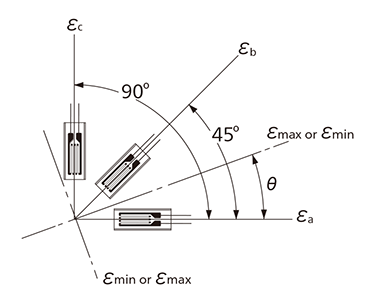
\includegraphics[width=3in]{images/Strain Gauge/Strain Gauge Orientation.png}
        \caption{Strain Gauge Orientation}
        \label{fig:Strain Gauge Orientation}
\end{figure}

\begin{gather}
    \varepsilon_{A} = (\frac{\varepsilon_{x} + \varepsilon_{y}} {2}) +  (\frac{\varepsilon_{x} - \varepsilon_{y}} {2})\cos({2\theta_{A}}) + \varepsilon_{xy}\sin({2\theta_{A}}) \\
    \varepsilon_{B} = (\frac{\varepsilon_{x} + \varepsilon_{y}} {2}) +  (\frac{\varepsilon_{x} - \varepsilon_{y}} {2})\cos({2\theta_{B}}) + \varepsilon_{xy}\sin({2\theta_{B}})\\
\varepsilon_{C} = (\frac{\varepsilon_{x} + \varepsilon_{y}} {2}) +  (\frac{\varepsilon_{x} - \varepsilon_{y}} {2})\cos({2\theta_{C}}) + \varepsilon_{xy}\sin({2\theta_{C}})
\end{gather}

\end{center} 


Electrically, strain gauges are resistors whose resistance changes based on how they deform.
This resistance change can be measured by a Wheatstone bridge.
\vspace{1em}

A Half-Bridge I configuration was chosen.
\begin{figure}[H]
    \centering
    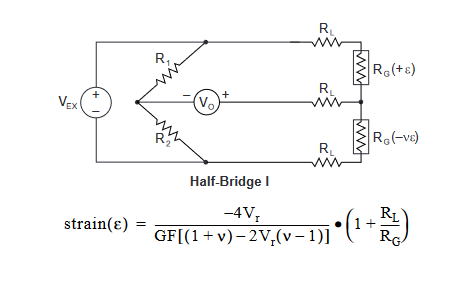
\includegraphics[width=5in]{images/calculating strain.png}
    \caption{Half-Bridge Resistor/Strain Gauge Configuration}
    \label{fig:hbi}
\end{figure}

\subsection{Strain Gauge Amplifier}
Since the voltage difference produced by a strain gauge in a Wheatstone bridge is very small (usually in a millivolts range), a strain gauge amplifier is used to amplify the voltage difference.
\vspace{1em}

For our strain gauge amplifier board, the HX711 was chosen because it is able to be powered off of 3.3V.
Additionally, we were able to find many reference schematics of HX711's used in strain gauge amplifiers, which aided in the development of our amplifier board.
\begin{figure}[H]
    \centering
    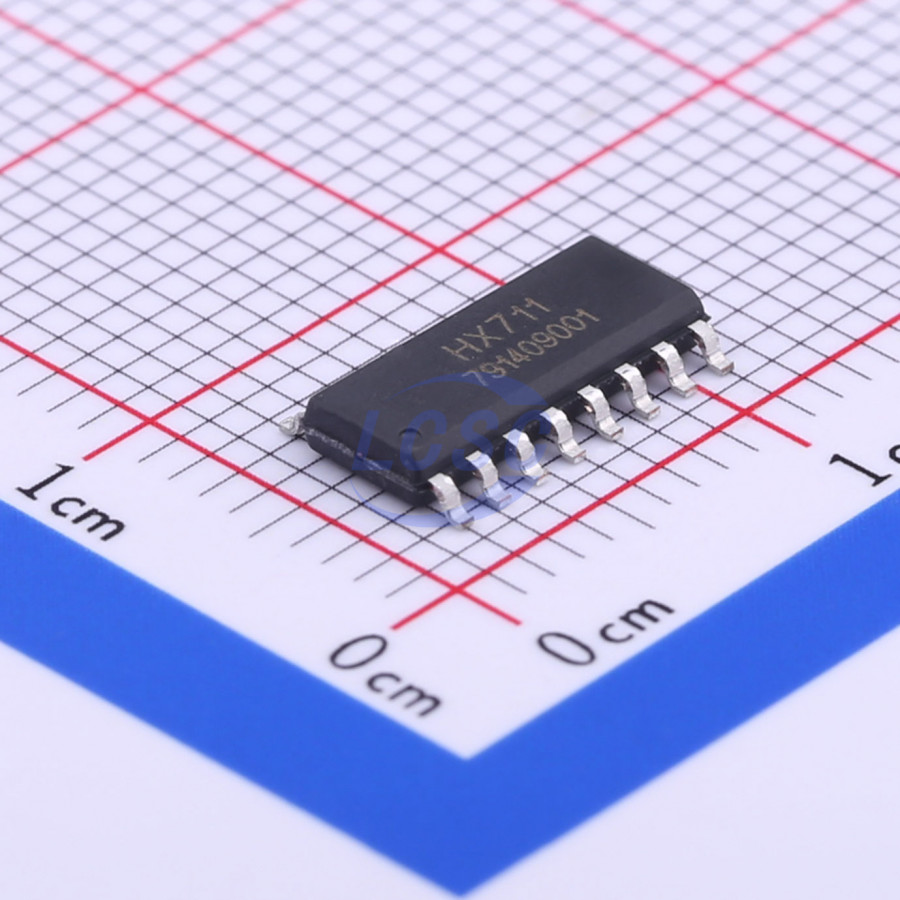
\includegraphics[width=2in]{images/hx711.jpg}
    \caption{HX711}
    \label{fig:hx711-pic}
\end{figure}

\subsection{Brake Pressure Sensor}
To measure the front and rear brake pressure, a media-isolated pressure transducer is used.
The brakes subteam selected for us Honeywell's MIPAG1XX050BSAAX.
This ratiometric sensor can measure pressure up to 50 bar, and uses a sealed gage pressure reference.
Its transfer function is defined to as
\begin{gather}\label{eq:bps}
    V_O = \frac{0.8\times V_S}{P_{max}-P_{min}}\times(P_{applied}-P_{min})+0.1\times V_S
\end{gather}
Where $V_O$ is the output voltage in V, $V_S$ is the voltage supply in V, $P_{applied}$ is the measured pressure, and $P_{max},P_{min}$ are the maximum and minimum pressures defined as $0.9\times V_S$ and $0.1\times V_S$ respectively.

It is important to note that this sensor runs off of 5V, so a voltage divider to step the maximum output down to 3.3V is required for the Teensy 4.0 to interface with it.
Additionally, the specific sensor model chosen interfaces with a Aptiv Metri Pack 150 connector.
\begin{figure}[H]
    \centering
    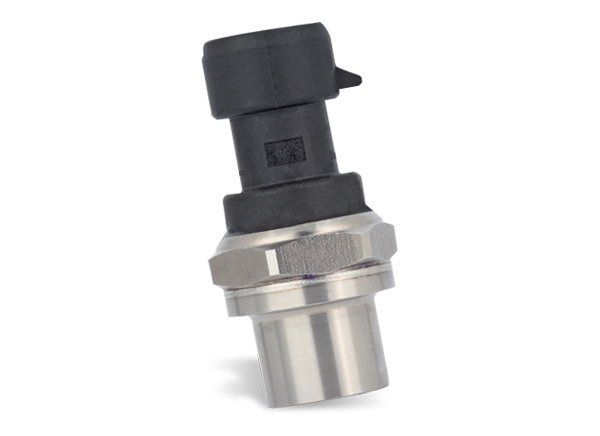
\includegraphics[width=2in]{images/mips.png}
    \caption{Honeywell MIPAG1XX050BSAAX}
    \label{fig:mips}
\end{figure}

\subsection{GPS Module}
A GPS module is used to collect data about SDM-23's position and velocity.
This can then be used to calculate laps and lap times, get a good idea of the top speed, and relate data channels such as lateral acceleration to track location.
The module used is the Adafruit Ultimate GPS Breakout, pictured in \ref{fig:gps} which is built around the MTK3339 chipset.

It is important to note that the position data is in degrees and minutes in the following format:
\begin{itemize}
    \item Latitude: DDMM.MMMM
    \item Longitude: DDDMM.MMMM
\end{itemize}
Interally these are stored as floating-point numbers.
These can be converted into decimal degrees by
\begin{gather}
    D_{decimal} = D+M/60
\end{gather}
Where $D$ and $M$ are the degrees and minutes values obtained from the module, and $D_{decimal}$ is decimal degrees.
\begin{figure}[H]
\centering
    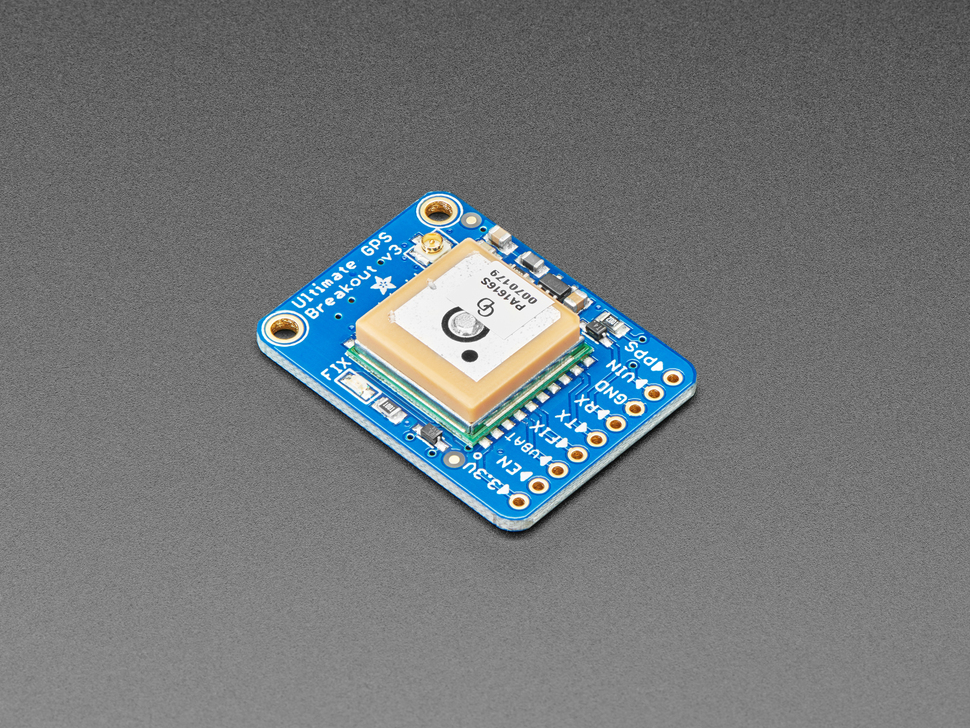
\includegraphics{images/gps.jpg}
    \caption{Adafruit Ultimate GPS Breakout}
    \label{fig:gps}
\end{figure}
An active external antenna is also used to increase the GPS Module's gain.
